\documentclass[11pt]{article}
\usepackage[a4paper, hmargin={2.8cm, 2.8cm}, vmargin={2.5cm, 2.5cm}]{geometry}
\usepackage{eso-pic} % \AddToShipoutPicture
\usepackage{graphicx} % \includegraphics
\usepackage{tabto}
\usepackage{enumerate}
\usepackage{txfonts}
\usepackage{graphicx}
\usepackage{float}
\usepackage{amsmath}
\usepackage{listings}
\usepackage{xcolor}
\lstset { %
    language=C++,
    backgroundcolor=\color{black!5}, % set backgroundcolor
    basicstyle=\footnotesize,% basic font setting
}


%% Change `ku-farve` to `nat-farve` to use SCIENCE's old colors or
%% `natbio-farve` to use SCIENCE's new colors and logo.
\def \ColourPDF {include/ku-farve}

%% Change `ku-en` to `nat-en` to use the `Faculty of Science` header
\def \TitlePDF   {include/ku-en}  % University of Copenhagen

\title{
  \vspace{3cm}
  \Huge{Some Title} \\
  \Large{More elaborate subtitle}
}

\author{
  \Large{Bjarke Kingo Iversen}
  \\ \texttt{bjarkekingo50@gmail.com} \\\\
  \Large{Susanne Truong}
  \\ \texttt{suzze-t@hotmail.com}
}

\date{
    \today
}

\begin{document}

\AddToShipoutPicture*{\put(0,0){\includegraphics*[viewport=0 0 700 600]{\ColourPDF}}}
\AddToShipoutPicture*{\put(0,602){\includegraphics*[viewport=0 600 700 1600]{\ColourPDF}}}

\AddToShipoutPicture*{\put(0,0){\includegraphics*{\TitlePDF}}}

\clearpage\maketitle
\thispagestyle{empty}

\newpage

%% Write your dissertation here.
\section{Abstract}
\newpage
\tableofcontents
\newpage
%%%%%%%%%%%%%%%%%%%%%%%%%%%%% Introduction %%%%%%%%%%%%%%%%%%%%%%%%%%%%%
\section{Introduction}
It is widely known that it can be time-consuming to choose the wrong path, if you want to travel from one city to another. It will most certainly be faster to aboard the train from Chicago to Seattle, rather than going through Los Angeles before heading to Seattle. Choosing the right path will therefore save a lot of time.\\
The problem herein is that its in lots of cases is nowhere intuitive which path that guarantees the consumation of time to be minimal. We probably can't withstand the big amounts of information if we should compute the shortest path, through millions of combinations by ourselves. For computersystems to choose such a path, they'd need a method for calculating such, an algorithm.\\
Different shortest-path algorithms are known to solve such problems theoretically. We'll examine the theory behind these, and analyse the complexity to see whether the time-complexity given by Bellmann-Ford and Dijkstras algorithms holds in real life implementations, by implementing them with both a binary and a fibonacci-heap in C++, thus finally to match them all up against each other.\\
We'll as well analyse and implement the A*-algorithm to see how well dijkstra match up against this on euclidean planar graphs. Since we're primarily interested in road-maps, we won't consider negative weights.\\

\section{Problem definition}
To examine and benchmark the complexity of different shortest-path algorithms, e.g. Dijkstra, Bellmann-Ford, and A* Search. We will do this by implementing and comparing them using different data structures and libraries. Finally we will compare the results of these experiments with the theoretical bounds.

%%%%%%%%%%%%%%%%%%%%%%%%%%%%%%% Notation %%%%%%%%%%%%%%%%%%%%%%%%%%%%%%%
\section{Notation}
A short list of notations used throughout the thesis:
\begin{itemize}
\item $G(V,E)$ = Graph, consisting of set of vertices V, and set of edges E
\item $s$ = Designated to be the source vertex s
\item $w(u,v)$ = Weighted distance from vertix u to v
\item $d[v]$ = The weigth of the current shortest path from s to v. $d[v]$ is initlized to be $\infty$ for all vertices besides the source vertex. $d[s]$ is initialized to be 0.
\item $\pi[v]$ = Predecessor/parent vertex to v in the current shortest path. $\pi[v]$ is initialized to be NIL. This is set to a vertex once/if a path is discovered from s to v.
\item $\delta(u,v)$ = the weigth of the shortest path from u to v.
\item lg(n) = $log_{2}$(n).
\item $v_{1}, v_{2}, ..., v_{k}$ a path from some start-vertice containing k vertices in successing order.
\item $h(v)$ = Heuristic function used on vertex v, for a more detailed description see section 11.1
\end{itemize}

%%%%%%%%%%%%%%%%%%%%%%%%%%% Shortest Paths %%%%%%%%%%%%%%%%%%%%%%%%%%%
\section{On Shortest Paths}
In the shortest path problem, a graph $G = (V,E)$ is given, where $V$	
is the set of vertices, and $E$ is the set of edges. Each edge
connects two vertices and contains a weight, indicating the cost of
moving between these vertices. By using a shortest path algorithm, we
can find a shortest path $P = {v_{1}, v_{2}, ..., v_{k}} \in V$ from a
given source vertex $s \in V$ to all other vertices $v \in V$. I.e.,
we want to find a path, where the total weight of the visited edges is
minimal.\\
We can compute the total sum of weights in a path P containing k vertices thus:\\
$$w(P) = \displaystyle\sum_{i=1}^{k} w(v_{i-1},v_i)$$

%%%%%%%%%%%%%%%%%%%%%%%%%%%%% Relaxation %%%%%%%%%%%%%%%%%%%%%%%%%%%%%
\noindent
\subsection{Initialization \& Relaxation}
When searching for the shortest path from a source vertex $s$ to a
vertex $v$, a shortest-path estimate $d[v]$ is preserved for each
vertex $v \in V$. To initialize the estimate and predecessor for all vertices, the following function is used:\\

\textbf{INITIALIZE-SINGLE-SOURCE$(G, s)$}
\begin{enumerate}
\NumTabs{24}
\setlength\itemsep{0em}
\item \textbf{for } each vertex $v \in G.V$
\item \tab{$d[v] = \infty$}
\item \tab{$\pi[v] = NIL$}
\item $d[s] = 0$
\end{enumerate}
The shortest-path estimate for the source is 0, since this is where the algorithm begins. The other vertices' distance is set to $\infty$, since the path from $s$ to a vertex $v$ is unknown at start. Not knowing the path also results in the predecessor being unknown, which is why $\pi[v]$ is set to NIL.\\
At first, $d[v]$ will be an overestimate, but if we see that the shortest path to $v$ can be improved by going through a vertex $u$, we update the estimate $d[v]$ with the new and lower cost. As better paths are found, we will eventually get the correct estimate and find the shortest path, if it exists. This technique is called relaxation and is used by the three algorithms that we will talk about later. The pseudocode for relaxing an edge $(u,v) $ is shown below:\footnote{Introduction to Algorithms, pg. 649}\\

\textbf{RELAX$(u, v, w)$}
\begin{enumerate}
\NumTabs{24}
\setlength\itemsep{0em}
\item \textbf{if } $d[v] > d[u] + w(u,v)$
\item \tab{$d[v] = d[u] + w(u,v)$}
\item \tab{$\pi[v] = u$}
\end{enumerate}
If the current distance from a source to the vertex $v$ is larger than the path going through vertex $u$ to $v$, the estimate is updated. And the predecessor for $v$ will then be $u$. The figure below illustrates the procedure of relaxing an edge $(u,v)$. Before relaxing the edge, we have that $d[v] > d[u] + w(u,v)$. $d[v]$ therefore gets decreased. Had the condition not been true, $d[v]$ would have remained at the same value of 10. 

\begin{figure}[H]
\centering
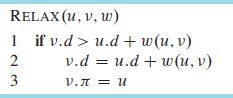
\includegraphics[scale=0.4]{relaxation.png}
\caption{Relaxing an edge $(u,v)$}
\end{figure}


%%%%%%%%%%%%%%%%%%%%%%%%%%%%% Properties %%%%%%%%%%%%%%%%%%%%%%%%%%%%%
\section{Properties of shortest path algorithms}
The shortest path algorithms that we have talked about will always find a shortest path, if it exists. This can be proved by looking at the properties that shortest paths and relaxation have. CLRS\footnote{Introduction to Algorithms, pg. 650} describes the following properties, that we may sometimes refer to by name, later in the report:

\subsection{Triangle inequality}
The triangle inequality lemma is a geometric property of triangles which states that the sum of two lengths of any two sides must be greater than or equal to the remaining side. That is, for any triangle with sides $\{x,y,z\}$, we have that $z \leq x+y$.\\\\
Applied to the shortest path problem we have that for any edge $(u,v) \in E$, we have $\delta(s,v)\leq \delta(s,u) + w(u,v)$. Thus the shortest path from s to v must be less than or equal to the shortest path from s to u added to the weigth from u to v.\\
\subsection{Upper-bound property}
The upper-bound property says that our estimate for the shortest distance to v is always greater than or equal to the actual shortest path from s to v, for all vertices v$\in$ V.\\\\
That is $\forall v \in V.(d[v]\geq \delta(s,v))$. Once our estimate holds the actual value for the shortest path, the estimate never changes.\\
\subsection{No-path property} Corollary to the Upper-bound property.\\
If there is no path from s to v, then we always have $d[v] = \delta(s,v) = \infty$.\\
\subsection{Convergence property}
The convergence property ensures us that if we from s, at sometime has u to v is the shortest path in G for some u,v $\in$ V, and if the estimated shortest path to u actually is the shortest path, we'd then have (prior to relaxing the edge (u,v)) that the estimated shortest path to v must be the shortest path to v at all times afterward.\\\\
That is, if $s\rightsquigarrow u\rightarrow v$ is a shortest path, and if $d[u] = \delta(s,u)$, then $d[v] = \delta(s,v)$ is assured at all time afterward.\\
\subsection{Path-relaxation property}
Our path-relaxation property ensures that the relaxation of a shortest path p will derive that the distance to the k'th vertix in p is equal to the shortest path to vertix k.\\
Let $p = \{v_{1}, v_{2},\cdots ,v_{k}\}$ be a shortest path that goes from $v_{1}$ to $v_{k}$. If the edges are relaxed in the order $(v_{1},v_{2}), (v_{2},v_{3}), \cdots , (v_{k-1}, v_{k})$, then $d[v_{k}] = \delta(s,v_{k})$ once the whole path is relaxed \footnote{Shortest Paths: 6.006 Intro to Algorithms, March 30 2011, Recitation 14. MIT}.
\subsection{Predecessor-subgraph property}
The predecessor-subgraph/parent-subgraph property ensures that once the shortest path to v is computed for all vertices v, the predecessor subgraph is a shorted-paths tree rooted at s.\\\\
Such that once $\forall v \in V.(d[v] = \delta(s,v))$ the predecessor subgraph that contains all the vertices with a finite distance from s, but with only edges that connects v to $\pi[v]$ is a shortest-path tree\footnote{Shortest Paths: 6.006 Intro to Algorithms, March 30 2011, Recitation 14. MIT}.
\end{itemize}

%%%%%%%%%%%%%%%%%%%%%%%%%%%%% Bellman-Ford %%%%%%%%%%%%%%%%%%%%%%%%%%%%%
\section{Bellman-Ford algorithm}
Bellman-Ford algorithm solves the single-source shortest-path problem in the case where edge weights may be negative. If there is a negative cycle, the cost of the shortest path is decreased every time the algorithm runs through the negative cycle. By doing this numerous times, we can receive arbitrarily negative weights, thus making the cost undefined. If no such cycle is found, the algorithm succesfully computes the shortest paths from s to each vertex v $\in$ V by iteratively decreasing d[v] by relaxing edges $\in$ E until $\delta(s,v)$ is found.\\
The algorithm returns true if and only if the graph has no negative-weight cycles reachable from the source vertex. Otherwise it terminates and returns false upon finding such a cycle. The pseudocode for Bellman-Ford's algorithm can be seen below:\footnote{Introduction to Algorithms, pg. 651}\\

\textbf{BELLMAN-FORD$(G, w, s)$}
\begin{enumerate}
\NumTabs{24}
\setlength\itemsep{0em}
\item INITIALIZE-SINGLE-SOURCE$(G, s)$
\item $\textbf{for } i = 1 \textbf{ to } |V[G]| -1$
\item \tab{$\textbf{for }$ each edge $(u,v) \in E[G]$}
\item \tab{}\tab{RELAX(u, v, w)}
\item $\textbf{for }$ each edge $(u,v) \in E[G]$
\item \tab{$\textbf{if } d[v] > d[u] + w(u,v)$}
\item \tab{}\tab{\textbf{return } FALSE}
\item \textbf{return } TRUE
\end{enumerate}

\noindent The graph is initialized in line 1 by calling INITIALIZE-SINGLE-SOURCE. For each vertex $v \in G.V$, the function sets the shortest-path estimate to $\infty$ and predecessor to NIL. $d[s]$ is set to 0. The algorithm then runs through a loop $|V[G]|-1$ times, relaxing each edge in the graph (line 2 to 4). After the relaxation, the algorithm then checks for negative weight cycles (line 5 to 6) and terminates, returning either true or false. 

\subsection{Correctness of Bellman Ford's algorithm}
To prove that Bellman Fords algorithm work, we'll do a contradiction-proof.\\\\
\textbf{Theorem}: If the graph G has no negative cycles reachable from s, then the algorithm returns true, upon termination we have that $\forall v \in V. (d[v] = \delta(s,v))$. If G has a negative cycle the algorithm returns false.\\\\
If G has no negative cycles, we have upon termination that $\forall v \in V. (d[v] = \delta(s,v))$. The algorithm must return true at some point and we must have that: $$d[v] = \delta(s,v) \leq \delta(s,u) + w(u,v) \leq d[u] + w(u,v)$$\\\\
Let us assume that G has a negative cycle that is reachable from s. Let this negative cycle be $c = (v_0, v_1,...,v_k)$ where $v_0$ = $v_k$, thus we have that $$\displaystyle\sum_{i=1}^{k} w(v_{i-1}, v_i)} < 0$$
Let us for the purpose of reaching a contradiction assume that Bellman-Ford returns true. Then we'd have by the statement we made just before that $$d[v_i] \leq d[v_{i-1}] + w(v_{i-1},v_{i})$$ for $i$ up to $k$.\\
By summing up the inequalities in the cycle c, we will have that: $$\displaystyle\sum_{i=1}^{k} d[v_i]} \leq \displaystyle\sum_{i=1}^{k} (d[v_{i-1}] + w(v_{i-1}, v_i))}$$
Which can be derived to
$$\displaystyle\sum_{i=1}^{k} d[v_i]} \leq \displaystyle\sum_{i=1}^{k} d[v_{i-1}]} + \displaystyle\sum_{i=1}^{k} {w(v_{i-1}, v_i)}$$
But since $\sum_{i=1}^{k} d[v_i]}$ and $\sum_{i=1}^{k} d[v_{i-1}]}$ both covers the exact same cycle, we must have that 
$$\displaystyle\sum_{i=1}^{k} d[v_i]} = \displaystyle\sum_{i=1}^{k} d[v_{i-1}]}$$
We can therefore zero them out, thus we get
$$0 \leq \displaystyle\sum_{i=1}^{k} w(v_{i-1}, v_i)}$$
Which contradict to the assumption that we had a negative cycle.\\
Thus we can conclude that that we return true if G has no negative weighted cycles reachable from the source, and false otherwise.
\footnote(den her) %http://people.csail.mit.edu/alinush/6.006-spring-2014/mit-fall-2010-bellman-ford.pdf + CLRS?



%%%%%%%%%%%%%%%%%%%%%%%%%%%%%%%% Heaps %%%%%%%%%%%%%%%%%%%%%%%%%%%%%%%%%
\section{Heaps}
In the following section, we will describe the priority queues we use for our interpretation of the Dijkstra's and A* search algorithm.\\
\subsection{Binary Min-Heaps}
A binary heap is a tree-like data-structure, where each node contains 2 child nodes, in a complete balanced way, such that all levels of the tree, except the last one is filled, and if the last one is not complete, the nodes from the level are filled from left to right. The height of a tree containing n nodes is $\lfloor lg(n) \rfloor$. When the height of the tree grows linearly the amount of nodes therefor grow exponentially. The amount of nodes in af tree of height n would therefor be between $2^n$ and $2^{n+1}-1$. But lets use the approximation of $2^n$ for now. The figure below shows an example of a min-heap containing 10 nodes. The left picture shows it as a binary tree, while the right one shows it as an array. The height of our tree is $\lfloor lg(10) \rfloor = 3$.

\begin{figure}[H]
\centering
\includegraphics[scale=0.4]{hob+array.png}
\caption{Min-heap seen as a binary tree and an array.}
\end{figure}

\noindent By using the properties of the binary heap, we can compute some nodes, given an index thus:\\
%\begin{center}
%$$\pmb{Parent(i) = \lfloor i/2 \rfloor}$$\\
$$Parent(i) = \lfloor i/2 \rfloor$$
%\pmb{$Left(i) = 2i$}\\
$$Left(i) = 2i$$
%\pmb{$Right(i) = 2i+1$}\\
$$Right(i) = 2i+1$$
%\end{center}
In the binary min-heap we have that the value of the nodes are in decreasing order when moving from a leaf node, up through the parent-nodes. Symmetrically, we have that the values are in ascending order when moving down arbitrarily through the nodes. That is, we have for all nodes that Min-heap[Parent(i)] $\leq$ Min-heap[i].\\\\
For our shortest-path algorithms to work on the binary-heap datastructure, we need the following operations:
\subsubsection{Decrease-Key}
By calling our Relaxation we use the Decrease-Key method, which is the method of decreasing the value of a given node i, if our relaxation can improve the distance-estimate. It changes the value of node i to our key and as long as the Parent(i) is larger than i, it swaps i with Parent(i), and assigns the the index i to the index Parent(i).\\\\

\textbf{DECREASE-KEY(Min-Heap, i, key)}
\begin{enumerate}
\NumTabs{24}
\setlength\itemsep{0em}
\item Min-Heap[i] = key
\item \textbf{while } i $>$ 1 and Min-Heap[Parent(i)] $>$ Min-Heap[i]
\item \tab{\textbf{Swap}(Min-Heap[i], Min-Heap[Parent(i)])}
\item \tab{i = Parent(i)}
\end{enumerate}
\subsubsection{Insert}
Insertion is the method of inserting a new node into our min-heap.\\
When we insert, we add 1 extra space to our heap, and inserts it here.\\
We run our Decrease-Key again to have our new node have the right place in the Min-Heap.\\

\textbf{INSERT(Min-Heap, key)}
\begin{enumerate}
\NumTabs{24}
\setlength\itemsep{0em}
\item \textbf{Size}(Min-Heap) = \textbf{Size}(Min-Heap) + 1
\item Min-Heap[\textbf{Size}(Min-Heap)] = NIL
\item DECREASE-KEY(Min-Heap, \textbf{Size}(Min-Heap), key)
\end{enumerate}
\ \\
\noindent We can in the ordinary Dijkstras algorithm do this in a more clever way which will be discussed in the 'Running time analysis'-section
\subsubsection{Extract-Min}
By calling our \textbf{Extract-Min} we take out the Min-Heap[1], which is the root of our Min-Heap and will be guaranteed by Insert and Decrease-Key to have the minimum-value. When we do this, we put up our terminal node in the root, decreases the heap-size by 1 and balances it by swapping it with the smallest child-node recursively until we have it in the right spot.\\

\textbf{BALANCE-MIN-HEAP(Min-Heap, i)}
\begin{enumerate}
\NumTabs{24}
\setlength\itemsep{0em}
\item L = Left(i)
\item R = Right(i)
\item \textbf{if } L $\leq$ \textbf{Size}(Min-Heap) \textbf{and} (Min-Heap[L] $<$ Min-Heap[i])
\item \tab \textbf{then } smallest = L
\item \tab \textbf{else } smallest = i
\item \textbf{if } R $\leq$ \textbf{Size}(Min-Heap) \textbf{and} (Min-Heap[R] $<$ Min-Heap[smallest])
\item \tab \textbf{then } minimum = R
\item \textbf{if } minimum $\neq$ i
\item \tab \textbf{then } \textbf{Swap}(Min-Heap[i], Min-Heap[minimum])
\item \tab \tab BALANCE-MIN-HEAP(Min-Heap, minimum)
\end{enumerate}
\ \\

\textbf{EXTRACT-MIN(Min-Heap)}
\begin{enumerate}
\NumTabs{24}
\setlength\itemsep{0em}
\item \textbf{if } \textbf{Size}(Min-Heap) $<$ 1
\item \tab raise error "Heap underflow"
\item min = Min-Heap[1]
\item Min-Heap[1] = Min-Heap[\textbf{Size}(Min-Heap)]
\item \textbf{Size}(Min-Heap) = \textbf{Size}(Min-Heap) - 1
\item BALANCE-MIN-HEAP(Min-Heap, 1)
\item \textbf{return} min
\end{enumerate}
\subsubsection{Increase-Key}
Similar to the Decrase-Key operation we need a method for increasing the key for the A*-Search algorithm. It changes the value of a node i to our key, and as long as the any of the childs is smaller than i, it swaps with the minimum of these, and assigns the index of i to the minimum child of i.\\

\textbf{INCREASE-KEY(Min-Heap, i, key)}
\begin{enumerate}
\NumTabs{24}
\setlength\itemsep{0em}
\item Min-Heap[i] = key
\item \textbf{while } i $<$ $\lfloor$\textbf{Size}(Min-Heap)/2$\rfloor$ and \textbf{Min}(Min-Heap[\textbf{Left}(i)],Min-Heap[\textbf{Right}(i)]) $<$ Min-Heap[i]
\item \tab{\textbf{Swap}(Min-Heap[i], \textbf{Min}(Min-Heap[\textbf{Left}(i)],Min-Heap[\textbf{Right}(i)])}
\item \tab{i = \textbf{Min}(Min-Heap[\textbf{Left}(i)],Min-Heap[\textbf{Right}(i)])}
\end{enumerate}
%%%%%%%%%%%%%%% OBS ALT OM FIB HEAPS ER UDKOMMENTERET (fra \iffalse til \fi)%%%%%%%%%%%%%%%
\iffalse
\subsection{Fibonacci-Heaps}
A Fibonacci heap is a collection of min-heap-ordered trees, though unlike the binary heap, which is ordered, the trees within the Fibonacci heaps are rooted but unordered.\footnote{Introduction to Algorithms, section 20.1}\\
\subsubsection{Use of circular doubly linked lists}
A Fibonacci heap may have multiple roots, but the minimum element of the heap is just one of the roots.\\
Each node n have a pointer \textbf{Parent}(n) to its parent, and a pointer \textbf{Child}(n) to any of its children. The children of n are thus linked together in a circulare doubly linked list, lets call it \textbf{Child-list(n)}, thus that each child m in Child-list(n) has pointers \textbf{Left}(m) and \textbf{Right}(m) that points to the m's left and right siblings. The last and first element in Child-list(n) therefore points to eachother. If node n only has one child m, then \textbf{Left}(m) = \textbf{Right}(m) = m. The order of siblings apperance in a list of children is arbitrary.\footnote{Introduction to Algorithms, section 20.1}\\
\textbf{BILLEDE AF FIB-HEAP + POINTERS (SOM PÅ SIDE 478)}\\\\
For our Fibonacci-heap to work properly we need a couple of more methods for information:
\begin{itemize}
\item \textbf{Min}(FIB-MIN-HEAP) = Pointer to the minimum element of FIB-MIN-HEAP.
\item \textbf{Degree}(n) = \textbf{Size}(\textbf{Child-list}(n)).
\item \textbf{Mark}(n) = Returns a boolean value that indicates whether a given node n has lost a child since the last time n was made the child of another node.
\end{itemize}
Marking is primarily for complexity-purposes which will be discussed in the Running-Time Analysis section.\\
Newly created nodes are unmarked, and a node n becomes unmarked whenever it is made the child of another node. Until we call the function \textbf{FIB-DECREASE-KEY} in section 9.2.2, we will just set all \textit{mark} fields to FALSE.\footnote{Introduction to Algorithms, section 20.1}\\
\newpage
\subsubsection{Fibonacci-Heap Operations}
For our shortest-path algorithms to work on the Fibonacci-heap datastructure, we need the following operations:
\subsubsection{Fib-Insert}
Insertion is our method of inserting a new node into the Fibonacci-heap.\\
Since we insert a node as a root, we need to check whether our new node would be the minimum element in the heap.\\\\
\textbf{FIB-INSERT}(FIB-MIN-HEAP, n)
\begin{enumerate}
\NumTabs{24}
\setlength\itemsep{0em}
\item Degree(n) = 0
\item Parent(n) = NIL
\item Child(n) = NIL
\item Left(n) = n
\item Right(n) = n
\item Mark(n) = FALSE
\item FIB-MIN-HEAP $\cup$ n
\item \textbf{if } \textbf{Min}(FIB-MIN-HEAP) = NIL \textbf{or } key[n] $<$ key[\textbf{Min}(FIB-MIN-HEAP)]
\item \tab \textbf{then } \textbf{Min}(FIB-MIN-HEAP) = n
\item \textbf{Size}(FIB-MIN-HEAP) = \textbf{Size}(FIB-MIN-HEAP) + 1
\end{enumerate}

\subsubsection{Fib-Extract-Min}
Upon extracting the minimum element n from the heap we set the childs of n to be root-nodes in the heap. If n wassn't the only node in the heap, we set the \textbf{Min}(FIB-MIN-HEAP) to \textbf{Right}(n) and call \textbf{CONSOLIDATE}, which iteratively links nodes together if we can find two roots n and m that has the same \textbf{Degree}, and where key(n) $\leq$ key(m). The minimum node we set before calling \textbf{CONSOLIDATE} may not be the node with the real minimum value.\\\\
\textbf{FIB-EXTRACT-MIN}(FIB-MIN-HEAP)
\begin{enumerate}
\NumTabs{24}
\setlength\itemsep{0em}
\item n = \textbf{Min}(FIB-MIN-HEAP)
\item \textbf{if } n $\neq$ NIL
\item \tab \textbf{then } \textbf{for } each child m of n
\item \tab \tab \tab \textbf{do } FIB-MIN-HEAP $\cup$ m
\item \tab \tab \tab \tab \textbf{Parent}(m) = NIL
\item \tab \tab \tab n' = \textbf{Right}(n)
\item \tab \tab \tab Remove n from FIB-MIN-HEAP
\item \tab \tab \tab \textbf{if } n == n'
\item \tab \tab \tab \tab \textbf{then } \textbf{Min}(FIB-MIN-HEAP) = NIL
\item \tab \tab \tab \tab \textbf{else } \textbf{Min}(FIB-MIN-HEAP) = n'
\item \tab \tab \tab \tab \tab \textbf{CONSOLIDATE}(FIB-MIN-HEAP)
\item \tab \tab \tab \textbf{Size}(FIB-MIN-HEAP) = \textbf{Size}(FIB-MIN-HEAP) - 1
\item \textbf{Return } n
\end{enumerate}
As mentioned the \textbf{CONSOLIDATE} ensures that none of the roots in the heap has the same Degree. We do the consolidating part by creating a new array and.........\\\\
\textbf{FIB-LINK}(FIB-MIN-HEAP, m, n)
\begin{enumerate}
\NumTabs{24}
\setlength\itemsep{0em}
\item Remove m from FIB-MIN-HEAP
\item \textbf{Child-list}(n) $\cup$ m
\item \textbf{Degree}(n) = \textbf{Degree}(n) + 1
\item \textbf{Mark}(m) = FALSE
\end{enumerate}
\\\\
\textbf{CONSOLIDATE}(FIB-MIN-HEAP)
\begin{enumerate}
\NumTabs{24}
\setlength\itemsep{0em}
\item \textbf{}
\end{enumerate}
\fi
\newpage
%%%%%%%%%%%%%%%%%%%%%%%%%%%%%%% Dijkstra %%%%%%%%%%%%%%%%%%%%%%%%%%%%%%%
\section{Dijkstra's algorithm}
Dijkstra's algorithm takes a weighted graph $G = (V, E)$ and finds the shortest path from a single source to each other vertex in the graph. To keep track of the vertices, the algorithm maintains two sets of vertices. The set $S$ consists of vertices, where the optimal shortest-path estimate from the source $s$ has been figured. The other set $Q$ is a minimum priority queue that contains the remaining vertices, i.e. $Q = V - S$. The algorithm will repeatedly extract a vertex with the minimum shortest-path estimate from $Q$ and add it to $S$, until all vertices have been discovered. If the graph happens to be connected, then for all $v \in V $, a vertex $v$ will be reachable from another vertex $w$ through an edge. If the graph is disconnected, some vertices will be unreachable, thus making some shortest paths infinite, if we try to reach these vertices.\\

\noindent 
\textbf{Assumptions}\\
For Dijkstra's algorithm to work, we must assume that the graph contains no negative weights. Once a vertex has been extracted from the min-priority queue, Dijkstra's algorithm will assume that the shortest path to that vertex has been found. This means the algorithm will never have to relax this vertex again. However, if there is a negative-weighted edge somewhere, the algorithm may find a wrong shortest-path.\footnote{http://stackoverflow.com/questions/13159337/why-doesnt-dijkstras-algorithm-work-for-negative-weight-edges} An example can be seen in the following figure:\\

\begin{figure}[H]
\centering
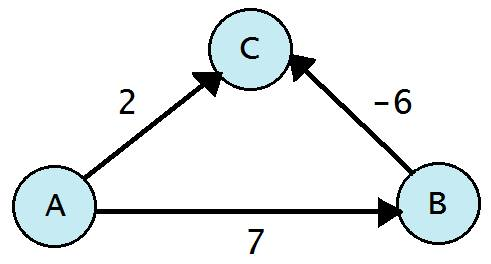
\includegraphics[scale=0.3]{neg-weight.png}
\caption{A graph with negative weights}
\end{figure}

\noindent In this figure, the graph consists of three vertices $A, B,$ and $C$. Dijkstra's algorithm starts at the source $A$ and will first extract $C$, since it has the shortest-path estimate of 2. Afterwards, the algorithm extracts the last vertex $B$ and terminates. Had it however tried to relax the negative edge between $B$ and $C$, a shorter path of $7 - 6 = 1$ would have been discovered. The result is therefore incorrect due to dijkstra utilizing the greedy property of \textbf{Lemma 1}, thus that $\forall (u,v) \in E.(w(u,v) \geq 0)$. \\

\noindent The pseudocode for Dijkstra's algorithm can be seen below:\footnote{Introduction to Algorithms, pg. 658}\\

\textbf{DIJKSTRA$(G, w, s)$}
\begin{enumerate}
\NumTabs{24}
\setlength\itemsep{0em}
\item INITIALIZE-SINGLE-SOURCE$(G, s)$
\item $S = $ \O
\item $Q = G.V$
\item $\textbf{while } Q \neq$ \O
\item \tab{$u = $ EXTRACT-MIN$(Q)$}
\item \tab{$S = S \cup \{u\}$}
\item \tab{\textbf{for} each vertex $v \in G.Adj[u]$}
\item \tab{}\tab{RELAX$(u,v,w)$}
\end{enumerate}

\noindent The graph is initialized in line 1 by calling INITIALIZE-SINGLE-SOURCE. For each vertex $v \in G.V$, the function sets the shortest-path estimate to $\infty$ and predecessor to NIL. $d[s]$ is set to 0. Dijkstra's algorithm maintains two sets, $S$ and $Q$. The set $S$ contains the vertices, whose final shortest-path estimates have been determined. In the beginning, no paths have been determined and thus $S$ will be empty (line 2). The min-priority queue $Q$ contains the vertices, whose shortest paths have not been found yet and is keyed by the vertices' current shortest-path estimates. In other words, the set of vertices in the graph is equal to the two sets, $V = S + Q$. $Q$ will contain all vertics in the graph at start (line 3).\\

\noindent We want to find $d[v]$ for all vertices, so Dijkstra's algorithm runs until the priority queue is empty. While $Q$ is not empty, the algorithm extracts the vertex with lowest $d[v]$ from $Q$ and adds it to the set $S$ (line 4 to 6). Afterwards, we examine for each vertex $v$ adjacent to $u$ if the shortest path found so far can be enhanced by taking the path through $u$. This is done by relaxing the edge $(u,v)$ (line 7 to 8).\\


%%%%%%%%%%%%%%%%%%%%%%%%% Dijkstra  modified %%%%%%%%%%%%%%%%%%%%%%%%%
\subsection{Dijkstra's algorithm - modified}
\noindent The original pseudocode finds the shortest path from a source vertex to all other vertices. We are only interested in finding the shortest path for a single target. so we have modified the original pseudocode for Dijkstra's algorithm. As soon as the algorithm finds the shortest path to the target vertex, it will terminate. This will reduce the amount of vertices visited, unless the target happens to be the last vertex found.\\

\textbf{MODIFIED-DIJKSTRA$(G, w, s, t)$}
\begin{enumerate}
\NumTabs{24}
\setlength\itemsep{0em}
\item $d[s] = 0$
\item $S = Q = \{s\}$
\item $\textbf{while } Q \neq  $ \O
\item \tab{$u = $ EXTRACT-MIN$(Q)$}
\item \tab{\textbf{if } $u = t$}
\item \tab{}\tab{\textbf{Terminate}}
\item \tab{\textbf{for} each vertex $v \in G.Adj[u]$}
\item \tab{}\tab{\textbf{if } $v \notin S$}
\item \tab{}\tab{}\tab{$S = S \cup \{v\}$}
\item \tab{}\tab{}\tab{$Q = Q \cup \{v\}$}
\item \tab{}\tab{}\tab{$d[v]  = d[u] + w(u,v)$}
\item \tab{}\tab{}\tab{$\pi[v] = u$}
\end{enumerate}

\noindent The pseudocode now takes a 4th parameter $t$, indicating the target vertex we want to find. Instead of calling the function \textit{INITIALIZE-SINGLE-SOURCE}, we only set the source's shortest-path estimate to 0. All other vertices are already assumed to have a shortest-path estimate equal to $\infty$, so it is not necessary to initialize the estimates to $\infty$.\\

\noindent The set $S$ no longer contains the vertices, whose final shortest-path estimates have been found. Instead, the set $S$ now consists of vertices $v$ for which a path to $v$ has been considered. By subtracting $S$ from $V$, we would get the set of vertices where $d[v]=\infty$ in the original Dijkstra's algorithm. The min-priority queue $Q$ has also been modified. Instead of adding all vertices in the graph, we only want to insert new vertices into the queue as they are discovered.\\ 

\noindent At start, $s$ is added to the sets $S$ and $Q$, since only the path to the source has been discovered and considered (line 2). Line 4 extracts a vertex $u$ with the minimum shortest-path estimate. If the vertex $u$ is the target vertex, the algorithm terminates. Else, the algorithm examines each vertex $v$ that is adjacent to $u$ in line 7. If $v$ has not been examined before, it will not be an element of $S$ or $Q$. Thus, we add $v$ to $S$ and $Q$. After this, the edge $(u,v)$ is relaxed, since $d[v]=\infty$ prior to being found and the predecessor is set to $u$.\\\\
The following figure illustrates the difference between the two algorithms.\\
\begin{figure}[H]
\centering
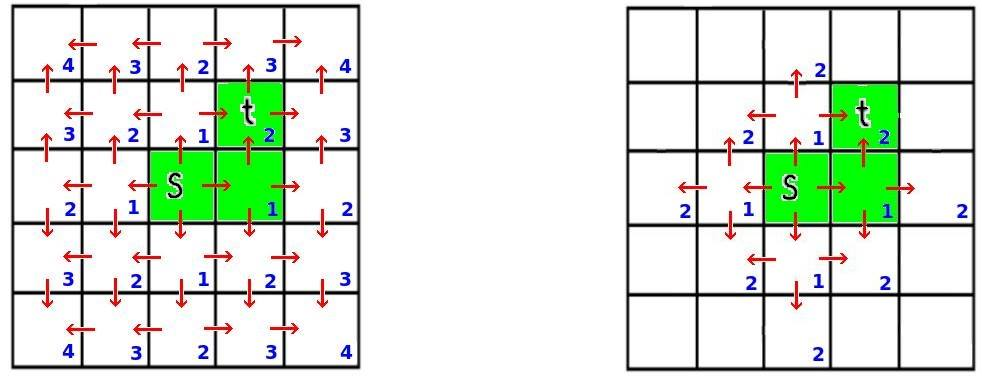
\includegraphics[scale=0.5]{dijkstra.png}
\caption{Dijkstra's algorithm vs. the modified Dijkstra's algorithm}
\end{figure}


%%%%%%%%%%%%%%%%%%%%%%%%%%%% Dijkstra proof %%%%%%%%%%%%%%%%%%%%%%%%%%%%
\subsection{Correctness of Dijkstra's algorithm}
To prove that Dijkstra's algorithm work, we will perform an induction proof. Let $S$ be the set of vertices, whose shortest path have been found, $S=V-Q$.\\

\noindent \textbf{Loop Invariant}\\
$\forall v\in S.(d[v] = \delta(s,v))$\\

\noindent \textbf{Initialization}\\
Let \textbf{Size}$(S)=1$. This is true when $S$ only holds the source vertex, $S = \{s\}$. Since $d[s]=0=\delta(s)$, the invariant holds.\\

\noindent \textbf{Maintenance}\\
Let $v$ be the latest vertex added to $S$. Let $S'$ = $S \cup \{v\}$. For each vertex in $S'$, we want to have that our loop invariant holds. EXTRACT-MIN(Q) ensures that the correct distance label gets extracted from $Q$ and put into $S$. We therefore only need to show that $d[v]=\delta(s,v)$ for $S'=S \cup \{v\}$. To prove this, we will perform a contradiction. Assume that there exists a shortest path $P^{sv}=(s, ..., v)$ from the source vertex $s$ to target vertex $v$ that has length $$w(P^{sv}) < d[v]$$
Before adding $v$ to $S$, the path $P^{sv}$ connects a vertex $u\in S$ to the vertex $v\in V-S$ through one or more edges. Since $v$ has not been added to $S$ yet, there must be one or more vertices on the path $P^{sv}$ that is in $V-S$. And since the source $s$ is in $S$, there must be one or more vertices on the path $P^{sv}$ that belongs to $S$. We can therefore define a vertex $y$ to be the first vertex along $P^{sv}$ that is an element of $V-S$. Let $x\in S$ be $y's$ predecessor along the path $P^{sv}$. Let $P^{sx}=(s, ..., x)$ be a subpath of $P^{sv}$ from vertex $s$ to $x$. This path is illustrated on figure~\ref{fig:eyy}. Since $x \in S$, we know by induction that $x$ got extracted with the correct shortest path distance $$d[x] \leq w(P^{sx})$$and that the edge $(x,y)$ got relaxed, so $$d[y] \leq d[x]+w(x,y) \leq w(P^{sx}) + w(x,y) \leq w(P^{sv})$$But we assumed $w(P^{sv}) < d[v]$ and $d[y] < d[v]$, which contradicts that EXTRACT-MIN returns a vertex $v$ from $V-S$ minimizing $d[v]$. $v$ has the shortest distance label, so $$d[v] \leq d[y]$$

\noindent \textbf{Termination}\\
We terminate once $Q = V-S =\O$. If $\exists t \in S$, we can backtrace the predecessors to obtain $\delta(s,t)$. Otherwise, we have that $\delta(s,t) = \infty$ by the no-path property.\\

\begin{figure}[H]
\centering
\includegraphics[scale=0.5]{SP.png}
\caption{An assumed shorter path from $s$ to $v$ going through the edge $(x,y)$.}
\label{fig:eyy}
\end{figure}

%%%%%%%%%%%%%%%%%%%%%%%%%%%%%%% A* search %%%%%%%%%%%%%%%%%%%%%%%%%%%%%%%
\section{A* search}
A* search algorithm was developed in 1968 and can be seen as a mix of Dijkstra's algorithm and Greedy Best-first search algorithm. 

\subsection{Greedy Best-First search}
\noindent beskrivelse af Greedy Best-first search... show example?



\noindent A* examines an edge only once, and like Dijkstra's, A* will favor vertices who are close to the source vertex. The downside of Dijkstra's is however that the target vertex' direction is unknown. Thus, it might consider paths going in the complete opposite direction.\\

\noindent Like the Greedy Best-first search algorithm, A* will also use heurestics to guide its search. The heuristic function can estimate how far away any vertex is from the goal. Vertices close to the goal are then favored over vertices who lie far away. However, Greedy Best-first search only uses the heuristic as information, when making a choice, making it a pure heuristic algorithm. By making a greedy decision based on only one criterion, the Best-first search algorithm runs considerably faster than Dijkstra's algorithm. The greedy solution is not always optimal though. By ignoring the distance moved so far, the algorithm may continue on a path it's on, even when the path has become very long.\\

\noindent A* does not perform a pure heuristic search, since it keeps the estimated distance from source to vertex in mind, before extending the path. A* will therefore not be as fast as Greedy Best-First search, but will at least guarantee that a shortest path is found. By combining the information that Dijkstra's and Best-First search uses, A* search will be at least as fast as Dijkstra's algorithm, since the search can go in a more precise direction. This makes us able to minimize the number of vertices visited, before the target vertex is found. \\

%%%%%%%%%%%%%%%%%%%%%%%%%%%%%% Heuristics %%%%%%%%%%%%%%%%%%%%%%%%%%%%%%
\subsection{Heuristic function for A* search}
A* will behave differently, depending on which heuristic function $h(v)$ we take in use. In the special case where $h(v)$ always gives 0, then only the shortest path estimate $d[v]$ will be looked at when a node is expanded. In this case, A* will be equal to Dijkstra's algorithm, since Dijkstra only considers $d[v]$. On the other hand, if $h(v)$ happens to be very high compared to $d[v]$, then only $h(v)$ is important. Thus, A* turns into Greedy Best-First-Search, since it will be a pure heuristic algorithm.\footnote{http://theory.stanford.edu/~amitp/GameProgramming/Heuristics.html}\\

\noindent If $h(v)$ is always smaller than or equal to the cost of moving from a vertex $v$ to the goal, then A* is assured to find a shortest path. When the  heuristic function $h(v)$ never overestimates the cost, the heuristic function is said to be admissible. An admissible heuristic can be seen as being too optimistic. It will make A* consider paths that are more costly than the shortest path. The smaller $h(v)$ is, the more nodes A* will expand, since the heuristic function is guiding the search in a less precise manner. It is therefore preferable to make $h(v)$ be as close as possible to the exact cost of moving from a vertex to the goal, since A* will run faster. \footnote{http://www.cs.colostate.edu/~anderson/cs440/index.html/doku.php?id=notes:week4c}\\

\noindent In the case where $h(v)$ is not admissible and overestimates the cost of moving from a vertex $v$ to the goal, A* can not guarantee to find a shortest path. On the other hand, A* can run even faster, since the search will be more specific, making A* expand less nodes. This property can for example be useful in games. If a computer is slow, computing a good path quickly may be preferable over computing an ideal path slowly.\\

\noindent Suppose we have a game, where the goal can be reached from going through a forest or flat land, and that the movement cost is 3 for the forest and 1 for flat land. A* thus expands over flat land three times as much as over the forest. If we for example decrease the movement cost on the forest from 3 to 2, A* will only expand twice as far along the flat land, compared to the forest. The shortest path will not be found, but on the good side we have increased the speed at which A* computes. \footnote{http://theory.stanford.edu/~amitp/GameProgramming/Heuristics.html}\\\\

\noindent \textbf{The Euclidean distance:}\\
\noindent The heuristic function we chose to use for A*, takes a vertex $v \in V$ and the destination vertex $t \in V$, and computes the Euclidean (i.e. straight-line) distance from $v$ to $t$. The Euclidean distance in a n-dimensional space on points $v$ and $t$ is computed by the following formula:\\
$$\sqrt{\displaystyle\sum_{i=1}^{n} (v_i - t_i)^2}$$
As we primarily consider plannar graphs, the Euclidean distance will be implemented using 2 dimensions, thus:\\
$$\sqrt{(v_x - t_x)^2 + (v_y - t_y)^2}$$
By using the Euclidean distance as our heuristic, we can guarantee that $h(v)$ will always be admissible. This is seen from the triangle equality ...\\

\noindent(write some more...)\\


%%%%%%%%%%%%%%%%%%%%%%%%% Pseudocode - A* search %%%%%%%%%%%%%%%%%%%%%%%%%
\subsection{Pseudocode for A* search algorithm}
We wish to find the shortest path to a single target, so the pseudocode is based on the pseudocode for the modified Dijkstra's algorithm.\\

\textbf{A* Search$(G, w, s, t)$}
\begin{enumerate}
\NumTabs{24}
\setlength\itemsep{0em}
\item $d[s] = 0$
\item $S = Q = \{s\}$
\item $\textbf{while } Q \neq  $ \O
\item \tab{$u = $ EXTRACT-MIN$(Q)$}
\item \tab{\textbf{if } $u = t$}
\item \tab{}\tab{\textbf{Terminate}}
\item \tab{\textbf{for} each vertex $v \in G.Adj[u]$}
\item \tab{}\tab{\textbf{if } $v \notin S$}
\item \tab{}\tab{}\tab{INCREASE-KEY$(Q, v, d[v] + h(v) ) $}
\item \tab{}\tab{}\tab{$S = S \cup \{v\}$}
\item \tab{}\tab{}\tab{$Q = Q \cup \{v\}$}
\item \tab{}\tab{}\tab{$d[v]  = d[u] + w(u,v)$}
\item \tab{}\tab{}\tab{$\pi[v] = u$}
\end{enumerate}
Like the modified Dijkstra's algorithm, A* search algorithm maintains two sets $S$ and $Q$. The set $S$ contains vertices $v$, for which a path to $v$ has been considered. As new vertices are discovered, they are also added to the min-priority queue $Q$. After adding a vertex $v$ to $S$ and $Q$, we then relax the edge and update the predecessor. To make sure that edges are relaxed properly, A* may only take non-negative edges.\\

\noindent Recall that Dijkstra's algorithm selects which vertex to visit next, by extracting the vertex with the lowest shortest-path estimate, $d[v]$ in the priority queue. The difference between Dijkstra and A* is that we now use heurestics to guide our search. A* search's priority queue is keyed by the current shortest path estimate $d[v]$ for each vertex $v$, added with the heuristic function $h(v)$. Each time A* search algorithm chooses which vertex to extract, it extracts the vertex $v$ with the lowest sum $d[v]+h(v)$.\\



\noindent  For A* search, the heuristic estimated cost $h(v)$ that we also want to examine, is gotten by taking the Euclidean distance  $\|t-v\|$ from a vertex $v$ to the target vertex $t$,  when $v$ is discovered (line 8). Thus, A* search will maintain a min-priority queue $Q$, where vertices are keyed by $w(s,v)+h(v)$ . To get this key, we use the function INCREASE-KEY to add the Euclidean distance to $d[v]$, (line 9). By repeatedly selecting the vertex with the lowest sum, we can get a more precise path search. This is illustrated in the following figure:\\

\begin{figure}[H]
\centering
\includegraphics[scale=0.45]{comparison.png}
\caption[]{Dijkstra's algorithm  vs  A* Search algorithm\footnotemark}
\end{figure}
\footnotetext{Amit P, Introduction to A*}

\noindent In this figure, the pink square represents the source vertex, while the dark blue square represents the target vertex. The other colored squares represent vertices who have been visited. Dijkstra's algorithm to the left has no estimation of how far away any vertex is, and thus expands in every direction, when trying to compute the shortest path to target. Meanwhile, A* keeps the Euclidean distance to the target in mind and thus favors vertices who lie south-east from the starting point. This rougly reduces the amount of vertices visited by half in the example, making A* much more efficient. 



%%%%%%%%%%%%%%%%%%%%%%%%%%%% A* search proof %%%%%%%%%%%%%%%%%%%%%%%%%%%%
\subsection{Correctness of A* search algorithm}
To prove that A* search algorithm work, we will perform an induction proof. Let $S$ be the set of vertices, whose shortest path have been found, $S=V-Q$. Let $g(u)$ be the shortest path from source to vertex $u$. Let $h(u)$ be the heurestic function that returns the Euclidean distance from vertex $u$ to target vertex.\\

\noindent \textbf{Loop Invariant}\\
$\forall v\in S.(d[v] = \delta(s,v))$\\

\noindent \textbf{Initialization}\\
Let \textbf{Size}$(S)=1$. This is true when $S$ only holds the source vertex, $S = \{s\}$. Since $d[s]=0=\delta(s)$, the invariant holds.\\

\noindent \textbf{Maintenance}\\
Let $v$ be the latest vertex added to $S$. Let $S'$ = $S \cup \{v\}$. For each vertex in $S'$, we want to have that our loop invariant holds. EXTRACT-MIN(Q) ensures that the correct distance label gets extracted from $Q$ and put into $S$. We therefore only need to show that $d[v]=\delta(s,v)$ for $S'=S \cup \{v\}$. Recall that EXTRACT-MIN(Q) returns a vertex $v$ with the lowest sum of $d[v]$ and $h(v)$. To prove $d[v]=\delta(s,v)$, we will therefore perform two contradictions. One for $h(v)$ and another for $d[v]$.\\

\noindent Let the heuristic function be the Euclidean distance from a vertex $u$ to $v$, $\|(u,v)\|$. Assume that there exists a path from $u$ to $v$ through a vertex $x$ that is less than the distance measured from $u$ to $v$. Thus, the heuristic function will have overestimated the distance from vertex v to target $t$. This can be seen as a triangle, where $$\|(u,v)\| > \|(u,x)\| + \|(x,v)\|$$\textbf{Lemma:} For any triangle, with sides $\{u,v,x\}$ we have that $\|v\| \leq \|u\| + \|x\|$.\\\\ From this lemma we have that any side of the triangle must be less than or equal to the remaining sides. But since we assumed that $\|(u,v)\| > \|(u,x)\| + \|(x,v)\|$ we must not have a triangle, and thus, we'd have a wrong meassurement for $\|(u,v)\|$. This is in contradiction with the original assumption that we had the euclidean distance $\|(u,v)\|$, and thus $$\|(u,v)\| \not > \|(u,x)\| + \|(x,v)\|$$
We can now derive that $$\|(u,v)\| \leq \|(u,x)\| + \|(x,v)\|$$which contradicts that we had a path from vertex u to v through x that would be less than $\|(u,v)\|$. Thus we have that the Euclidean distance from $u$ to $v$ is measured correctly and that the heuristic function $h(v)$ is admissible. If $h(v)$ is not admissible and  overestimates the cost, we would not be able to guarantee that a shortest path has been found. \\

\noindent For the next proof by contradiction, assume that there exists a shortest path $P^{sv}=(s, ..., v)$ from the source vertex $s$ to target vertex $v$ that has length $$w(P^{sv}) < d[v]$$
Before adding $v$ to $S$, the path $P^{sv}$ connects a vertex $u\in S$ to the vertex $v\in V-S$ through one or more edges. Since $v$ has not been added to $S$ yet, there must be one or more vertices on the path $P^{sv}$ that is in $V-S$. And since the source $s$ is in $S$, there must be one or more vertices on the path $P^{sv}$ that belongs to $S$. We can therefore define a vertex $y$ to be the first vertex along $P^{sv}$ that is an element of $V-S$. Let $x\in S$ be $y's$ predecessor along the path $P^{sv}$. Let $P^{sx}=(s, ..., x)$ be a subpath of $P^{sv}$ from vertex $s$ to $x$. Since $x \in S$, we know by induction that $x$ got extracted with the correct shortest path distance $$d[x] + h(x) \leq w(P^{sx}) + h(x)$$and that the edge $(x,y)$ got relaxed, so $$d[y]+h(y)$$ 
$$\leq \; d[x]+w(x,y)+h(y)$$
$$\leq \; w(P^{sx}) + w(x,y) + h(y)$$
$$\leq \; w(P^{sv})$$But we assumed $w(P^{sv}) < d[v]$ and $d[y] < d[v]$, which contradicts that EXTRACT-MIN returns a vertex $v$ from $V-S$ minimizing $d[v]$. $v$ has the shortest distance label, so $$d[v] \leq d[y]$$
\textbf{Termination}\\
We terminate once $Q = V-S =\O$. If $\exists t \in S$, we can backtrace the predecessors to obtain $\delta(s,t)$. Otherwise, we have that $\delta(s,t) = \infty$ by the no-path property.\\


%%%%%%%%%%%%%%%%%%%%%%%%% Implementation %%%%%%%%%%%%%%%%%%%%%%%%%%
\section{Implementation}
To examine the complexity of Dijkstra's, Bellman-Ford, and A* search algorithm, we have implemented them in C++. The code can be found in the appendix and we have used the following C++ libraries in our implementations:\footnote{http://www.cplusplus.com/reference/}

\begin{itemize}
\item $<$vector$>$
\item $<$queue$>$
\item $<$set$>$
\item $<$iostream$>$
\end{itemize}

\noindent The $<$vector$>$ library allows us to define vectors that represent arrays that can change in size. With vectors, adding or removing elements from its end is quite efficient. This is for example useful for saving predecessor pairs. When an algorithm discovers a new vertex, we want to save a new vector containing the vertex and its predecessor. Since the number of vertices discovered will vary from target to target, a dynamic array will therefore be useful.\\

\noindent The $<$queue$>$ library is used for our priority queue that contains pairs of integers. To store the pairs, we use the library $<$set$>$ that allows us to store the elements so they follow a certain order. Finally, we also want to print output to the terminal, such as the shortest path for a vertex. This can be done by using the library $<$iostream$>$.\\

\noindent The implementations take a graph and then runs until the target vertex has been found. When finished, we then call the functions print\textunderscore dist() and print\textunderscore path(). The function print\textunderscore dist() prints the shortest path distance, while print\textunderscore path() prints out the path taken from source to target vertex. The following algorithm PRINT-PATH illustrates how print\textunderscore path() works:\footnote{Introduction to Algorithms, pg. 601}\\ 

\textbf{PRINT-PATH$(G, s, v)$}
\begin{enumerate}
\NumTabs{24}
\setlength\itemsep{0em}
\item \textbf{if }$v == s$
\item \tab{print $s$}
\item \textbf{elseif }$v.\pi == NIL$
\item \tab{print "no path from $s$ to $v$ exists"}
\item \textbf{else } PRINT-PATH$(G, s, v.\pi)$
\item \tab{print $v$}
\end{enumerate}

\noindent The algorithm takes a graph $G$, source $s$, and target vertex $v$ as arguments. If target is equal to source, the source is printed. If $v$ has no predecessor, we print that no path from $s$ to $v$ exists. Else, we print the target $v$ and run the algorithm recursively, giving $v$'s predecessor as the target. The algorithm will then run until the predecessor is equal the source.\\

\subsection{Implementation of Dijkstra's algorithm}
We have a priority queue of datatype pair <int, int>. The vertex is stored as the second element, while the first element contains its distance from the source...


\subsection{Implementation of Bellman-Ford}
...
\subsection{Implementation of A* search}
...






%%%%%%%%%%%%%%%%%%%%%%%%% Running time analysis %%%%%%%%%%%%%%%%%%%%%%%%%%
\newpage
\section{Running time analysis}
We use the following notation for relevant running time complexities:
\begin{itemize}
    \item $O(n)$ = The upper bound of operations needed for some f(n) times a constant c. The number of operations needed is always less than or equal to n.
    \item $\theta(n)$ = The precise bound of operations needed for some f(n) times a constant c. The number of operations needed is always equal to n. 
\end{itemize}
We say that a function f(n) is upper bounded by a function g(n) asymptotically, if we for some n and ongoing have that f(n) $\leq$ g(n).\\
We say that a function f(n) is precise bounded by a function g(n) asymptotically, if we for some n and ongoing have that $c_1$ * g(n) $\leq$ f(n) $\leq$ $c_2$ * g(n).
\\\\
For the most accurate way of comparing we want to find the tightest bound g(n) close to f(n), so we have a somewhat precise meassurement for f(n). 
\subsection{Bellman Ford}
The Bellman Ford algorithm doesn't need no priority queue to work on, it simply relaxes all the edges V-1 times where V is the number of vertices in the graph. The implementation can choose to have some sort of data-structure i.e. 2 arrays:
\begin{itemize}
\item 1 containing the shortest-path distances at termination
\item 1 containing the predecessors upon termination
\end{itemize}
We can compute the running time of Bellman Ford's algorithm by looking at how many times we do each operation.\\
By looking at the pseudocode described in section 7 we see that Bellman-Ford primarily uses 3 operations, initialization of the graph, relaxation of edges and checks whether we have a negative-cycle.\\
The initialization step sets the predecessors and current distances to the vertex to infinity $\forall v. \in V \neq s$. This takes $\theta(V)$ time.\\ We relax all the edges in $\theta(E)$, as we relax a single edge in $\theta(1)$ time. We do this V-1 times and obtains the time of $\theta(E) * \theta(V)$. Finally we do E checks in $\theta(1)$ time, but we only do this as long as we have no negative-cycle, thus we have the checking part taking $O(E)$ time.\\
By addding them all up we obtain a running time of:\\
$\theta(V) + \theta(E*V) + O(E)$\\
By removing the small asymptotes we finally reach a running time of:\\
$\theta(E*V)$
\newpage
\subsection{Dijkstra}
The Dijkstra and the modified Dijkstra is bounded by 3 functions, defined in section 9.1; Decrease-key, Insertion and Extract-Min.
\subsubsection{Running time of Decrease-key}
The running time of a Decrease-key operation is bounded by the height of the binary tree, since we at worst case might decrease a leaf node and swap it all the way up in the root. We analysed the height of such a tree in section 9, and thus for a heap containing V vertices, a Decrease-key operation therefore takes $O(lg(V))$ time. 
\subsubsection{Running time of Insert}
In the modified Dijkstra we insert new vertices in the priority-queue whenever we found one. As we described in section 9.1.2, the insertion makes two constant operations followed by a call to Decrease-key we know takes $O(lg(V))$ time. Thus we have a running time of $O(lg(V))$ per insertion operation.\\\\
In the ordinary Dijkstra, we put all the vertices in V into a priority queue Q. In the initialization step we have that all vertices except the source is initially $\infty$, thus by putting in the source vertex s in Q as the root we can load V-1 vertices into Q arbitrarily.\\ Since we have that $\forall v \in V-\{s\}. (d[v] = \infty)$, we don't need to call any Decrease-key function. We therefore only make constant operations per vertice v, thus getting the running time of $\theta(1)$, per insertion.\\We use a constant operation for putting s into V, followed by V-1 insertions in constant time. Finally we will therefore get a running time of $\theta(V)$ for putting V vertices into Q.
\subsubsection{Running time of Extract-Min}
The running time of the Extract-Min function is bounded by the height of the binary tree as discussed in section 12.2.1. The running time is highly depended on Balance-Min-Heap, which makes at most $lg(V)$ swaps for V vertices, thus getting a complexity of $O(lg(V))$.
\subsubsection{Final running time}
\textbf{Modified Dijkstra}\\
The final running time of the modified Dijkstra can be computed by looking at how many times we do each operation.\\
We know that we for V vertices, in worst case do V insertions. Thus getting $O(V) * O(lg(V)) = O(V*lg(V))$. If we had the worst case of V insertions, we possibly may do V Extract-min operations, if we don't find the target vertex t. Thus we have the running time of $O(V) * O(lg(V)) + O(V*lg(V))$ when added together with insertions. We have E edges, worst case, we must relax everyone of them and call Decrease-key E times. Thus we will have a complexity of $O(E) * O(lg(V)) = O(E*lg(V))$.\\\\
Adding all of them up, we have the running time of $O(V*lg(V)) + O(V*lg(V)) + O(E*lg(V)) = 2*O(V*lg(V)) + O(E*lg(V))$.\\
If we do not have an edge (v,u) per vertice v-1 we would have some vertice unreachable, thus it would never had been added to Q. This means that the number of edges is the dominant to the final running time. We can remove the constants, and the asymptotically small complexities to finally reach a running time of:\\
$O(E*lg(V))$\\\\
\textbf{Original Dijkstra}\\
The final running time of the original dijkstras algorithm can as well be computed by looking at the number of operations.\\
We load V vertices into Q with running time of $\theta(1)$ per insertion, thus getting the running time of $\theta(V)$. We have to do V Extract-min operations, which takes $\theta(V) * O(lg(V))$, thus we now have the running time of $\theta(V) + O(V*lg(V))$. Finally we would worst case call Decrease-key E times, which we computed to take $O(lg(V))$ time, thus we have a time of $O(E*lg(V))$ for decreasing keys.\\\\
Adding all of them up, we have the running time of $\theta(V) + O(V*lg(V)) + O(E*lg(V))$. As in the modified dijkstras algorithm analysis, we here also have that the numbers of edges is dominant to the numbers of vertices. We remove the asymptotic small complexities to finally reach a running time of:\\
$O(E*lg(V))$\\\\\\
\textbf{The difference}\\
We see that the running time of the modified dijkstras in worst case will be the running time of the original dijkstras. This is because that the destination point may be the last vertex to visit.\\
\subsection{A*-Search}
\textbf{NOTHING YET}
\newpage



\section{Results}
\section{Bibliography}
\section{Appendix}
\subsection{Implementation of Dijkstra-modified}
\begin{lstlisting}
#include <iostream>
#include <queue>
#include <set>
#include <vector>
using namespace std;

#define ii pair<int,int>

vector<ii> graph[100];
vector<ii> predecessor[100];
bool visited[100];
int dist[100];

/* Runs Dijkstra's algorithm until target vertex is found */
void dijkstra_modified(int vertices, int source, int target){
  //define priority queue pq
  set<ii> pq;
	
  //insert source vertex and mark it as visited
  pq.insert(ii(0, source));
  predecessor[source].push_back(ii(source, source));
  dist[source] = 0;
  visited[source] = 1;

  //While pq not empty
  while(!pq.empty()){
    //extract vertex u from priority queue
	ii u = *pq.begin();	
	int vertex_u = u.second;
		
	//if target found
	if (vertex_u == target){
	  return;
	}

	pq.erase(u);
	visited[vertex_u] = 1;

	//For each vertex v adjacent to u:
	for(int i = 0; i < graph[vertex_u].size(); i++){
	  //define vertex v and w(u,v)
	  int vertex_v = graph[vertex_u][i].second;
	  int weight_v = graph[vertex_u][i].first;

	  //if v has not been visited
	  if(visited[vertex_v] == 0){
//mark as visited and update pq + distance.
		visited[vertex_v] = 1;
		pq.insert(ii(dist[vertex_u] + weight_v , vertex_v));
		dist[vertex_v] = dist[vertex_u] + weight_v;

		//update predecessor
		predecessor[vertex_v].push_back(ii(vertex_u, vertex_v));
	  }

	  //if v has been visited, but another possible path (edge) was found
	  else {
		if (dist[vertex_v] > dist[vertex_u] + weight_v){
		  //update pq + distance
		  pq.erase(ii(dist[vertex_v], vertex_v));
		  pq.insert(ii(dist[vertex_u] + weight_v , vertex_v));
		  dist[vertex_v] = dist[vertex_u] + weight_v;
				
		  //update predecessor		
		  predecessor[vertex_v].pop_back();
		  predecessor[vertex_v].push_back(ii(vertex_u, vertex_v));		
		  }
		}
	}
  }
}

/* Print distance from source to target vertex*/
void print_dist(int dist[], int target){
	cout << dist[target] << endl;
}

/* Print path taken from source to target vertex */
void print_path(int source, int target){
	int pre = predecessor[target][0].first;
	int suc = predecessor[target][0].second;

	if (source == target){
		cout << source << endl;
	}
	else if (pre == 0){
		cout << "No path from source to vertex exists" << endl;
	}
	else {
		cout << suc << " <- ";
		print_path(source, pre);
	}
}


int main(){
	int vertices, edges, source, target;

	cout << "How many vertices in the graph?" << endl;
	cin >> vertices;
	
	cout << "How many edges in the graph?" << endl;
	cin >> edges;
	
	cout << "Weight of the edges?" << endl;
	for(int i = 0; i < edges ;i++){
		int x,y,w;
		cin >> x >> y >> w;
		graph[x].push_back(ii(w,y));
	}

	source = 1;
	target = 5;
	dijkstra_modified(vertices, source, target);
	
	cout << endl << "Path: " << endl;
	print_path(source, target);
	cout << endl << "Total distance: " << endl;
	print_dist(dist, target);
	
	return 0;
}
\end{lstlisting}

\end{document}
